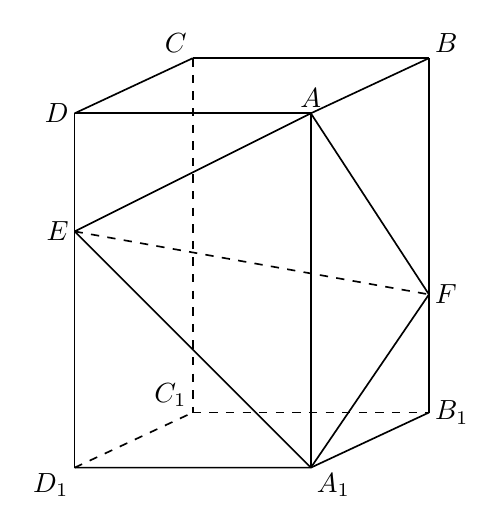
\begin{tikzpicture}[x=1cm,y=1cm,font=\normalsize,
  geometry edge/.style={draw=black,solid,line width=.6pt},
  geometry edge dashed/.style={draw=black,dashed,line width=.6pt},
  geometry label/.style={font=\normalsize,inner sep=2pt}]
\coordinate (D) at (0.00,4.50);
\coordinate (C) at (1.50,5.20);
\coordinate (B) at (4.50,5.20);
\coordinate (A) at (3.00,4.50);
\coordinate (E) at (0.00,3.00);
\coordinate (F) at (4.5,2.2);
\coordinate (D1) at (0.00,0.00);
\coordinate (C1) at (1.5,0.7);
\coordinate (B1) at (4.5,0.7);
\coordinate (A1) at (3.00,0.00);
\draw[geometry edge] (D)--(A);
\draw[geometry edge] (C)--(B);
\draw[geometry edge] (D)--(C);
\draw[geometry edge] (B)--(A);
\draw[geometry edge] (A)--(E);
\draw[geometry edge] (A)--(F);
\draw[geometry edge] (A)--(A1);
\draw[geometry edge] (E)--(A1);
\draw[geometry edge] (F)--(A1);

\draw[geometry edge] (D)--(E);
\draw[geometry edge] (E)--(D1);
\draw[geometry edge] (D1)--(A1)--(B1);
\draw[geometry edge] (B)--(B1);
\draw[geometry edge dashed] (C)--(C1);
\draw[geometry edge dashed] (C1)--(B1);
\draw[geometry edge dashed] (D1)--(C1);
\draw[geometry edge dashed] (E)--(F);
\node[geometry label,left] at (D) {$D$};
\node[geometry label,above left] at (C) {$C$};
\node[geometry label,above right] at (B) {$B$};
\node[geometry label,above] at (A) {$A$};
\node[geometry label,left] at (E) {$E$};
\node[geometry label,right] at (F) {$F$};
\node[geometry label,below left] at (D1) {$D_1$};
\node[geometry label,above left] at (C1) {$C_1$};
\node[geometry label,right] at (B1) {$B_1$};
\node[geometry label,below right] at (A1) {$A_1$};
\end{tikzpicture}
